\documentclass[12pt]{article}
\usepackage{amsmath}
\usepackage{graphicx}
\usepackage{adjustbox}
\usepackage{booktabs}
\usepackage{tabularx}
\usepackage{fullpage}
\usepackage{subcaption}
\usepackage{cite}
\usepackage{float} % Added to allow [H] float specifier



\title{Spatio-Temporal Machine Learning for Economic Forecasting: A Cross-Indicator and Cross-Country Analysis Using World Bank Data}
\author{Jiadong Zhang\thanks{Email: \texttt{dereksodo@gmail.com}}}
\date{May 2025}

\begin{document}

\maketitle

\begin{abstract}
This paper develops a spatio-temporal framework for forecasting key macroeconomic indicators using machine learning techniques. Leveraging World Bank panel data from 1960 to 2020, we investigate three core tasks: (1) cross-indicator prediction—forecasting one major indicator based on others; (2) national-level time series forecasting; and (3) cross-national forecasting for major economies. Through comparative analysis of models including XGBoost, Random Forest, and linear baselines, we find that most structural indicators are highly predictable, while GDP growth remains volatile and difficult to model. We introduce a novel feasibility rate metric to assess reliability across multiple performance dimensions. Our results highlight both the promise and the limitations of data-driven methods in economic forecasting and underscore the importance of model selection, data context, and indicator stability.
\end{abstract}

\newpage
\tableofcontents
\newpage


\section{Introduction}

Macroeconomic indicators provide a comprehensive lens for assessing the economic and social development of countries. This study leverages World Bank panel data from 1960 to 2020 to identify key national indicators and evaluate their predictability using machine learning. The focus is on cross-indicator prediction: can one major indicator be reliably predicted from the others?
\section{Literature Review}

Recent advancements in machine learning (ML) have significantly influenced macroeconomic forecasting. This section reviews key studies that have explored the integration of ML techniques into economic prediction models.

\subsection{Nonlinearity and Regularization in ML Forecasting}

Goulet Coulombe et al. (2019) investigate the efficacy of ML in macroeconomic forecasting, emphasizing the importance of capturing nonlinear relationships in economic data. Their study concludes that nonlinearity is a crucial factor in improving forecast accuracy. They also highlight that traditional factor models serve as effective regularization tools within ML frameworks, aiding in managing model complexity and preventing overfitting. The authors advocate for the use of K-fold cross-validation as a best practice for model evaluation and selection. Their findings suggest that ML models, when properly regularized and validated, can outperform traditional econometric models, especially during periods of economic uncertainty and financial stress \cite{GouletCoulombe2019}.

\subsection{Automating Forecasting with ML Techniques}

Hall (2018) explores the application of ML methods to macroeconomic forecasting, focusing on the automation of model selection and parameter tuning. The study demonstrates that ML algorithms can process vast and complex datasets, identifying patterns that traditional models might overlook. Hall's analysis reveals that ML models can outperform both simple time-series models and consensus forecasts from professional economists, particularly in predicting short-term economic indicators like the unemployment rate. The research underscores the potential of ML to enhance forecasting accuracy by reducing reliance on manual model specification and expert judgment \cite{Hall2018}.

\subsection{ML Applications in China's GDP Forecasting}

Yang et al. (2024) apply various ML models to forecast China's quarterly real GDP growth, assessing their performance against traditional econometric models and expert forecasts. Their study finds that ML models generally achieve lower forecast errors, particularly during stable economic periods. However, during economic inflection points, expert forecasts may exhibit greater accuracy due to a more nuanced understanding of the macroeconomic environment. Additionally, the authors employ interpretable ML techniques to identify key variables influencing GDP fluctuations, providing insights into the underlying drivers of economic change \cite{Yang2024}.

\subsection{Synthesis and Implications for Current Research}

The reviewed studies collectively highlight the transformative impact of ML on macroeconomic forecasting. They demonstrate that ML models, with their ability to capture complex nonlinear relationships and process large datasets, can enhance forecast accuracy beyond traditional methods. These findings inform the current research by underscoring the importance of incorporating ML techniques into economic prediction models, particularly for analyzing cross-indicator relationships, time series data, and cross-country economic dynamics.
While the empirical studies reviewed above emphasize the technical advances of ML-based forecasting, it is equally important to align these findings with economic theory. For instance, the persistent unpredictability of GDP growth observed in both past studies and our own results echoes theoretical insights from the Solow growth model\cite{Solow1956}, which attributes long-term economic growth primarily to exogenous technological progress—a factor that is inherently difficult to observe or predict. Likewise, indicators such as life expectancy and energy consumption—which consistently achieve low RMSE/STD and MASE and high $R^2$ and DA—reflect long-term structural trends that are more stable and easier to model. The declining predictive value of agricultural output aligns with structural transformation theory, which explains the shift of economic activity from agriculture to industry and services as economies develop. By framing ML findings within established theoretical paradigms, this study highlights not only algorithmic performance but also its macroeconomic interpretability.\cite{Solow1956, Kuznets1971}

% This section should review key literature on macroeconomic forecasting using machine learning.
% Include comparisons of cross-indicator modeling, single-country time series forecasting, and international panel data approaches.
% Discuss how your work extends or differs from past studies such as Goulet Coulombe (2019), Hall (2018), and Yang et al. (2024).
\section{Data and Methods}

\subsection{Data Source}

\begin{itemize}
    \item World Bank Open Data, 1960--2020, including G20 expect African Union.
    \item Main dataset: [World Bank Data by Indicators](https://github.com/light-and-salt/World-Bank-Data-by-Indicators) (GitHub repository)
    \item We choose 40 features, 2 representative features each in 20 categories by the World Bank.\footnote{See src/utils.py/feature\_codes for 40 initial features}
Some data are missing, and we only choose features if more than 60\% of relevant data are present. After cleaning and imputation, Principal Component Analysis (PCA) was used to select 10 relatively independent indicators, denoted $\{F_1, F_2, \ldots, F_{10}\}$, each with a feature load denoting how well it can "predict" other indicators. \footnote{Check Table \ref{tab:indicator_table} for details.}
\end{itemize}

\begin{table}[H]
    \centering
    \small
    \adjustbox{center}{
        \begin{tabular}{|c|c|c|}
            \hline
            \textbf{Indicator Code} & \textbf{Indicator Name} & \textbf{Feature Loading} \\
            \hline
            SP.DYN.LE00.IN & Life expectancy at birth, total (years) & 0.36759578 \\
            SP.URB.TOTL.IN.ZS & Urban population (\% of total population) & 0.34436319 \\
            NV.AGR.TOTL.ZS & Agriculture, forestry, and fishing, value added (\% of GDP) & -0.34223186 \\
            EG.USE.PCAP.KG.OE & Energy use (kg of oil equivalent per capita) & 0.28370116 \\
            FS.AST.PRVT.GD.ZS & Assets of private sector banks to GDP (\%) & 0.22820370 \\
            NE.IMP.GNFS.ZS & Imports of goods and services (\% of GDP) & 0.19327803 \\
            NY.GDP.MKTP.CD & GDP (current US\$) & 0.18121013 \\
            NE.EXP.GNFS.ZS & Exports of goods and services (\% of GDP) & 0.16005320 \\
            NY.GDP.MKTP.KD.ZG & GDP growth (annual \%) & -0.12023558 \\
            EN.ATM.GHGT.KT.CE & Total greenhouse gas emissions (kt of CO$_2$  equivalent) & 0.08242521 \\
            \hline
        \end{tabular}
    }
    \caption{Indicator Table}
    \label{tab:indicator_table}
\end{table}




We have some explanations about this. Negative feature loadings in this context should be interpreted as showing the direction of contribution relative to other features, and they often reflect well-established economic phenomena—such as the declining share of agriculture in GDP with development, or the varying relationship between growth rates and structural economic factors.
The sign itself is not inherently meaningful on its own, but should be understood in the context of the overall model and dataset.

For “Agriculture, forestry, and fishing, value added (\% of GDP)”, a negative loading often reflects the empirical reality that, as countries develop, the relative contribution of agriculture to GDP typically decreases—even as the economy grows overall. In higher-income economies, agriculture forms a smaller percentage of total output. Thus, in a multivariate context, a negative loading may simply capture this pattern of structural transformation.

For “GDP growth (annual \%)”, a negative loading could indicate that, within the chosen principal component or regression direction, higher GDP growth rates are associated with lower values of the principal component or the target variable—perhaps due to cyclical effects, catch-up growth in developing economies, or statistical collinearity with other features in the dataset.

\subsection{Data Preprocessing}

\begin{itemize}
    \item Interpolated missing values for convenience.\footnote{See /src/feature\_engineering.py}
    \item Constructed a country-year-feature panel: each row is a unique (country, year) pair.
\end{itemize}



\subsection{Machine Learning Models}

The following models are compared\footnote{See /src/models.py for parameters}:
\begin{itemize}
    \item Linear Regression (LR)
    \item Ridge Regression
    \item Lasso Regression
    \item Elastic Net
    \item Support Vector Regression (SVR)
    \item Random Forest (RF)
    \item K-Nearest Neighbors (KNN)
    \item XGBoost
    \item Locally Weighted Regression (LWR)
\end{itemize}

\subsection{Experimental Setup}

\begin{itemize}
    \item \textbf{Year ranges:}
    \begin{itemize}
        \item Full period: 1960--2020
        \item Recent period: 2010--2020
    \end{itemize}
    \item \textbf{Cross-Validation:} 5-fold cross-validation is used for each prediction, averaging metrics across folds.
    \item \textbf{Evaluation Metrics:}
    \begin{itemize}
        \item Standardized error (RMSE/STD)
        \item Coefficient of Determination ($R^2$)
        \item Mean Absolute Scaled Error (MASE)
        \item Directional Accuracy (DA)
        \item \textbf{Feasibility Rate (Heuristic Indicator):} For each model and indicator, we define a feasibility score as the average proportion of cases where at least 3 out of 4 predictions fall within an acceptable region. Specifically, we compute:
        \begin{align*}
        \alpha_1 &= \mathbf{1}\left[\frac{\text{RMSE}_i}{\text{STD}_i} < 1\right] \\\\
        \alpha_2 &= \mathbf{1}\left[R_i^2 > 0.6\right] \\\\
        \alpha_3 &= \mathbf{1}\left[\text{MASE}_i < 1\right] \\\\
        \alpha_4 &= \mathbf{1}\left[\text{DA}_i > 0.7\right]
        \end{align*}
        \[
        \text{Feasibility Rate} = \frac{1}{N} \sum_{i=1}^N \mathbf{1}\left[ \sum_{j=1}^4 \alpha_i \geq 3\right]
        \]
        This indicator serves as a summary of how often a model’s predictions are statistically reliable according to our predefined thresholds. These thresholds---RMSE/STD $< 1$, $R^2$ $> 0.6$, MASE $< 1$, and DA $> 0.7$---are informed by conventions in time-series forecasting and model validation literature \cite{Hyndman2006, Shmueli2016, Goodwin1993, Kim2016}. For example, RMSE/STD $< 1$ is commonly interpreted as indicating better-than-baseline performance, and $R^2$ $> 0.6$ represents moderate-to-strong explanatory power in applied economic models. MASE $< 1$ is considered an effective threshold because it implies forecast accuracy superior to that of a naive benchmark \cite{Hyndman2006}. For Directional Accuracy (DA), values exceeding 0.7 are often regarded as strong evidence of directional predictability, especially in volatile economic environments where DA $= 0.5$ represents random guessing \cite{Goodwin1993, Kim2016}. While these binary thresholds simplify multidimensional performance into an interpretable heuristic, we recognize that they are not strict cutoffs but rather well-supported conventions in applied forecasting research. Moreover, potential overfitting is addressed via 5-fold cross-validation and consistent out-of-sample evaluation.
    \end{itemize}
    \item \textbf{Visualization:} For each model and year range, bar plots of the 4 metrics are generated, with feasible region thresholds indicated.
\end{itemize}

\section{Cross-Indicator Analysis}

\subsection{Prediction Task}
For each indicator $F_k$, we predict its value for each country-year using the remaining 9 indicators as input features. The process is repeated for all $k = 1, \ldots, 10$.
\subsection{Prediction Results}
% Retain your current performance evaluation here.

% Sample Figure Placeholders
\begin{figure}[h]
    \centering
    \begin{subfigure}[b]{0.48\textwidth}
        \centering
        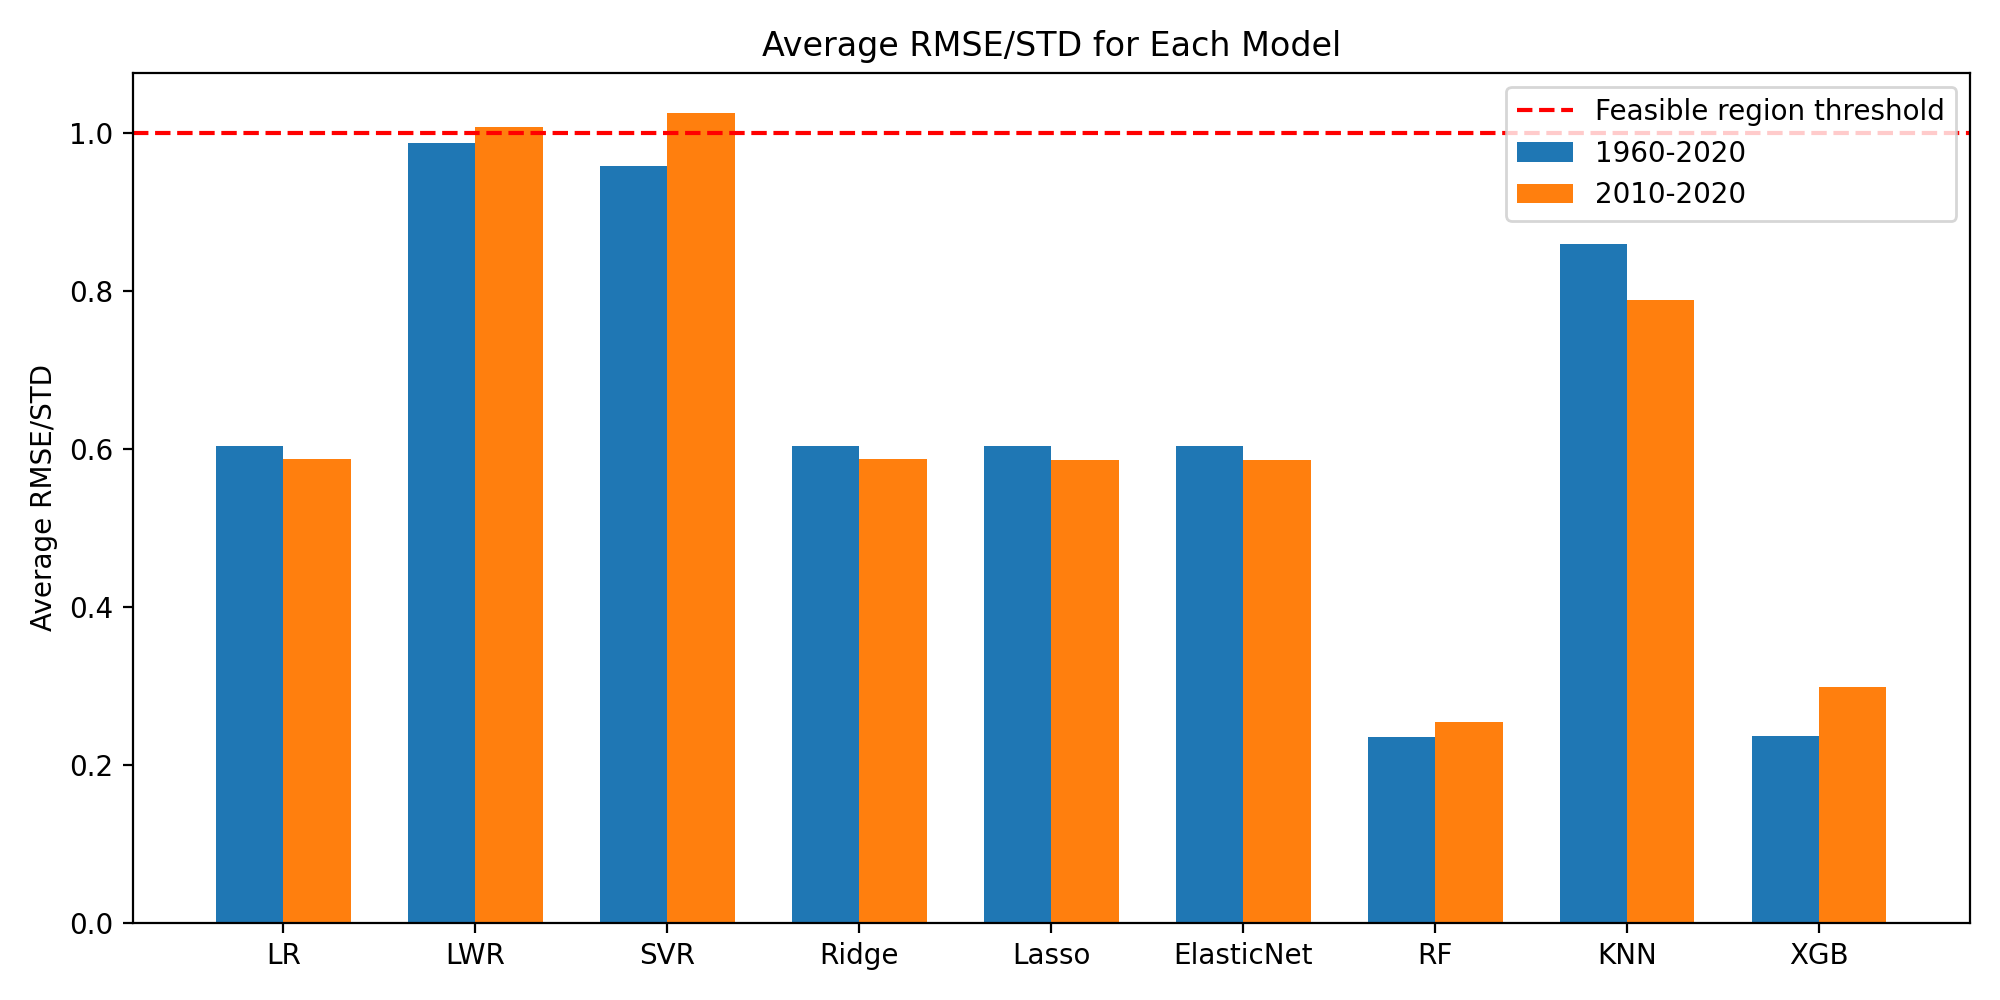
\includegraphics[width=\linewidth]{Average_RMSE_STD_figure1.png}
        \label{fig:rmse_std}
    \end{subfigure}
    \hfill
    \begin{subfigure}[b]{0.48\textwidth}
        \centering
        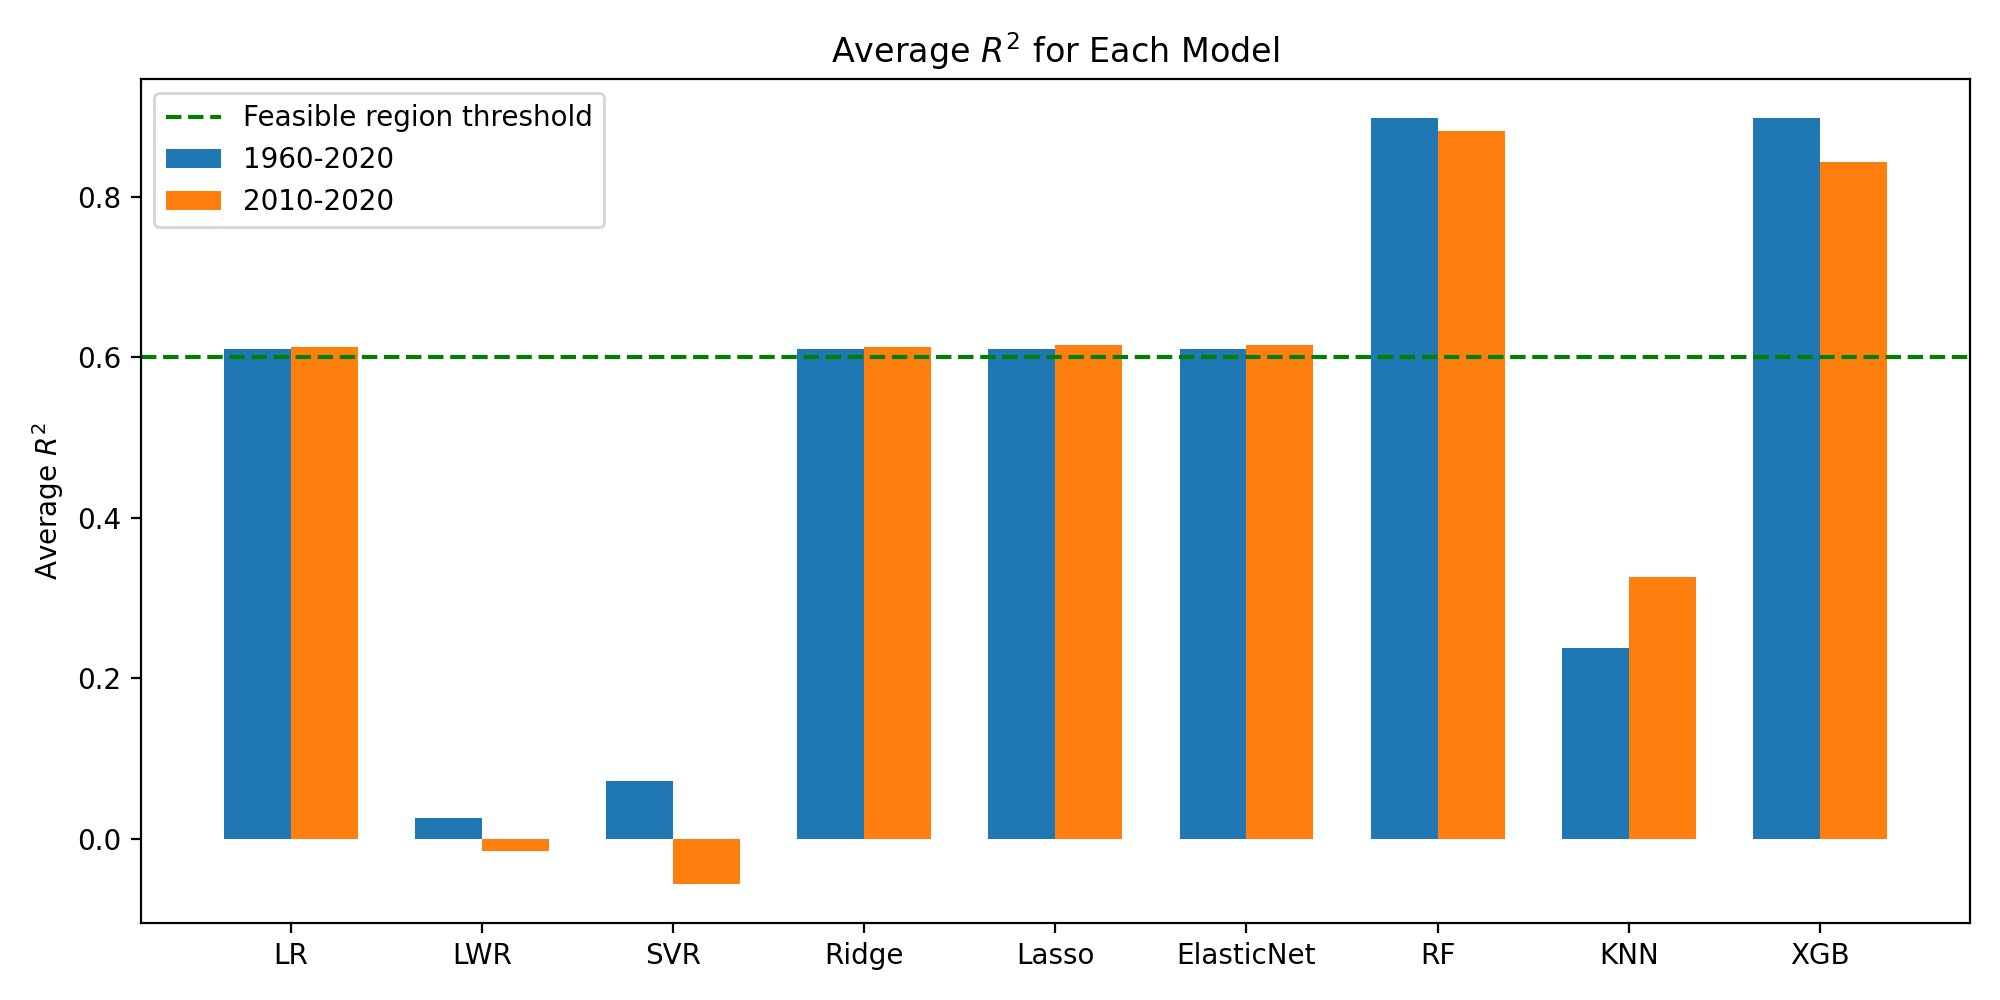
\includegraphics[width=\linewidth]{Average_R2_figure1.png}
        \label{fig:r2}
    \end{subfigure}
    \caption{Comparison of Model Performance: RMSE/STD and $R^2$ (1960–2020, 2010–2020)}
    \label{fig:model_compare_1}
\end{figure}
\begin{figure}[h]
    \centering
    \begin{subfigure}[b]{0.48\textwidth}
        \centering
        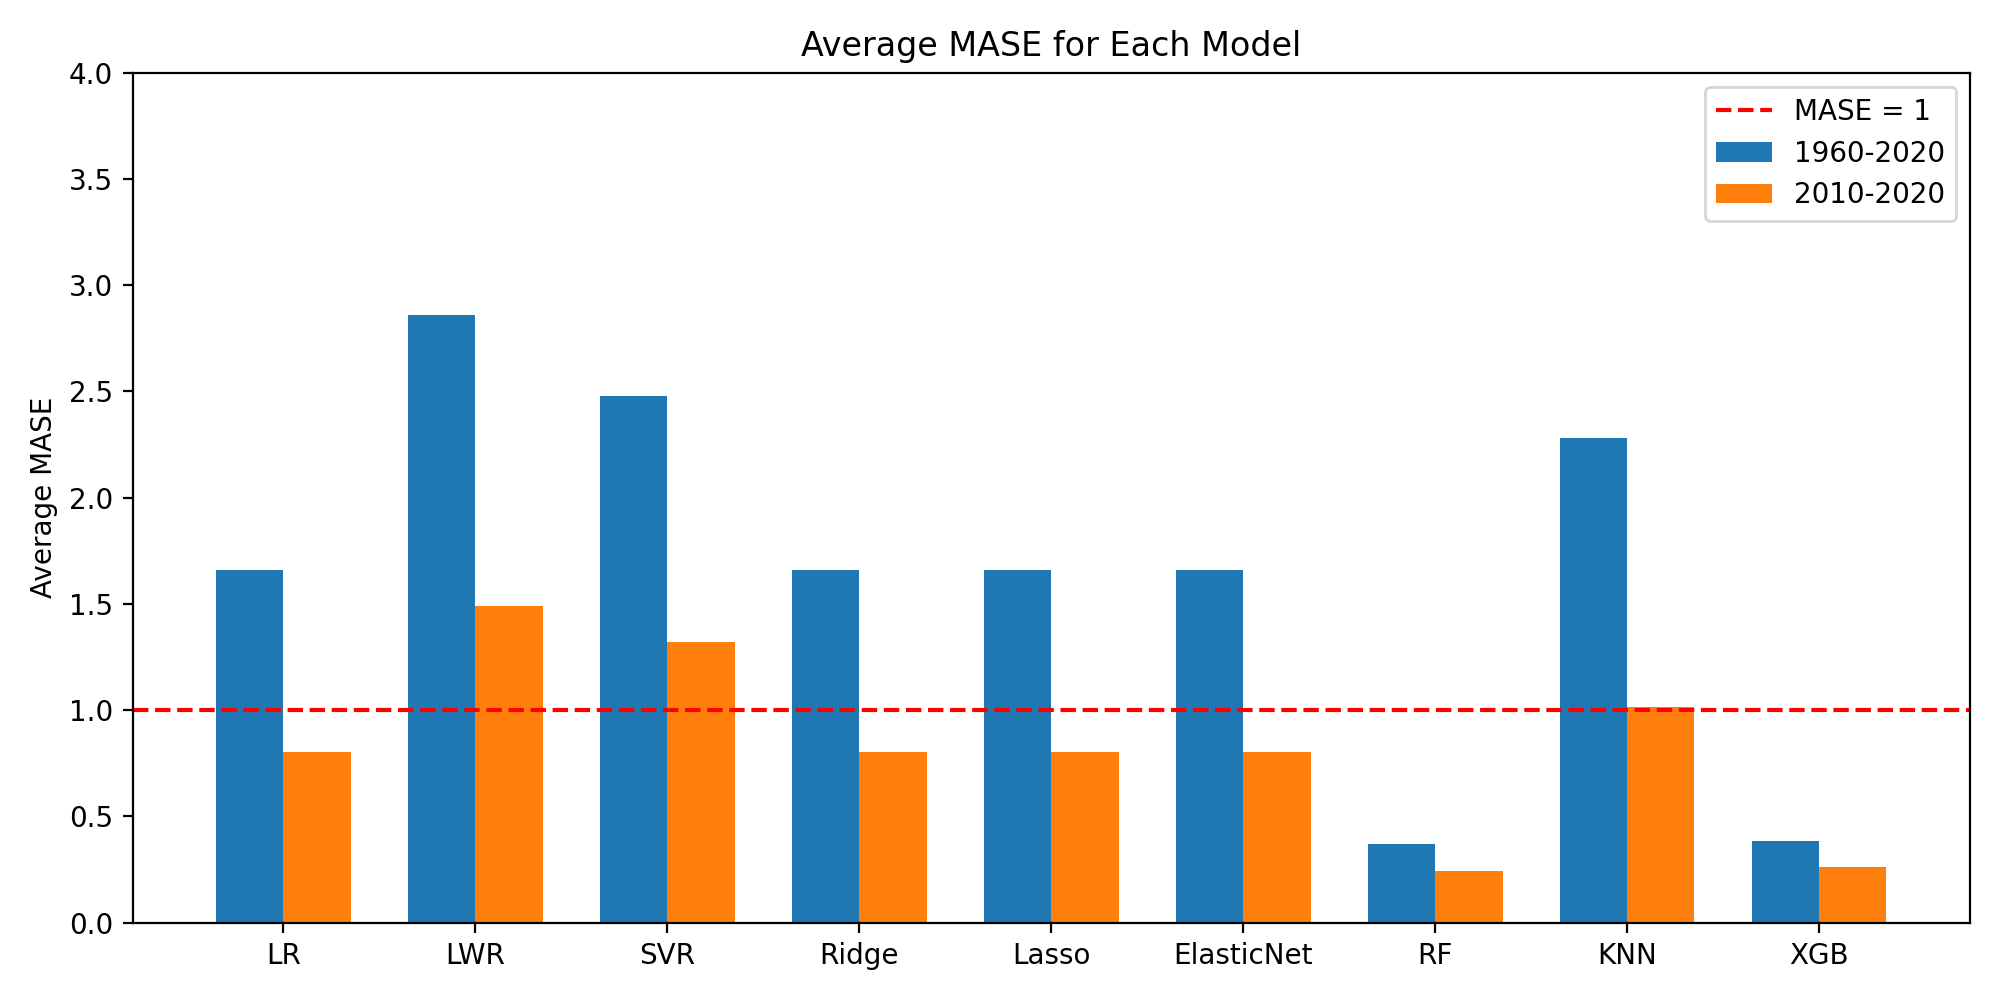
\includegraphics[width=\linewidth]{Average_MASE_figure2.png}
        \label{fig:MASE}
    \end{subfigure}
    \hfill
    \begin{subfigure}[b]{0.48\textwidth}
        \centering
        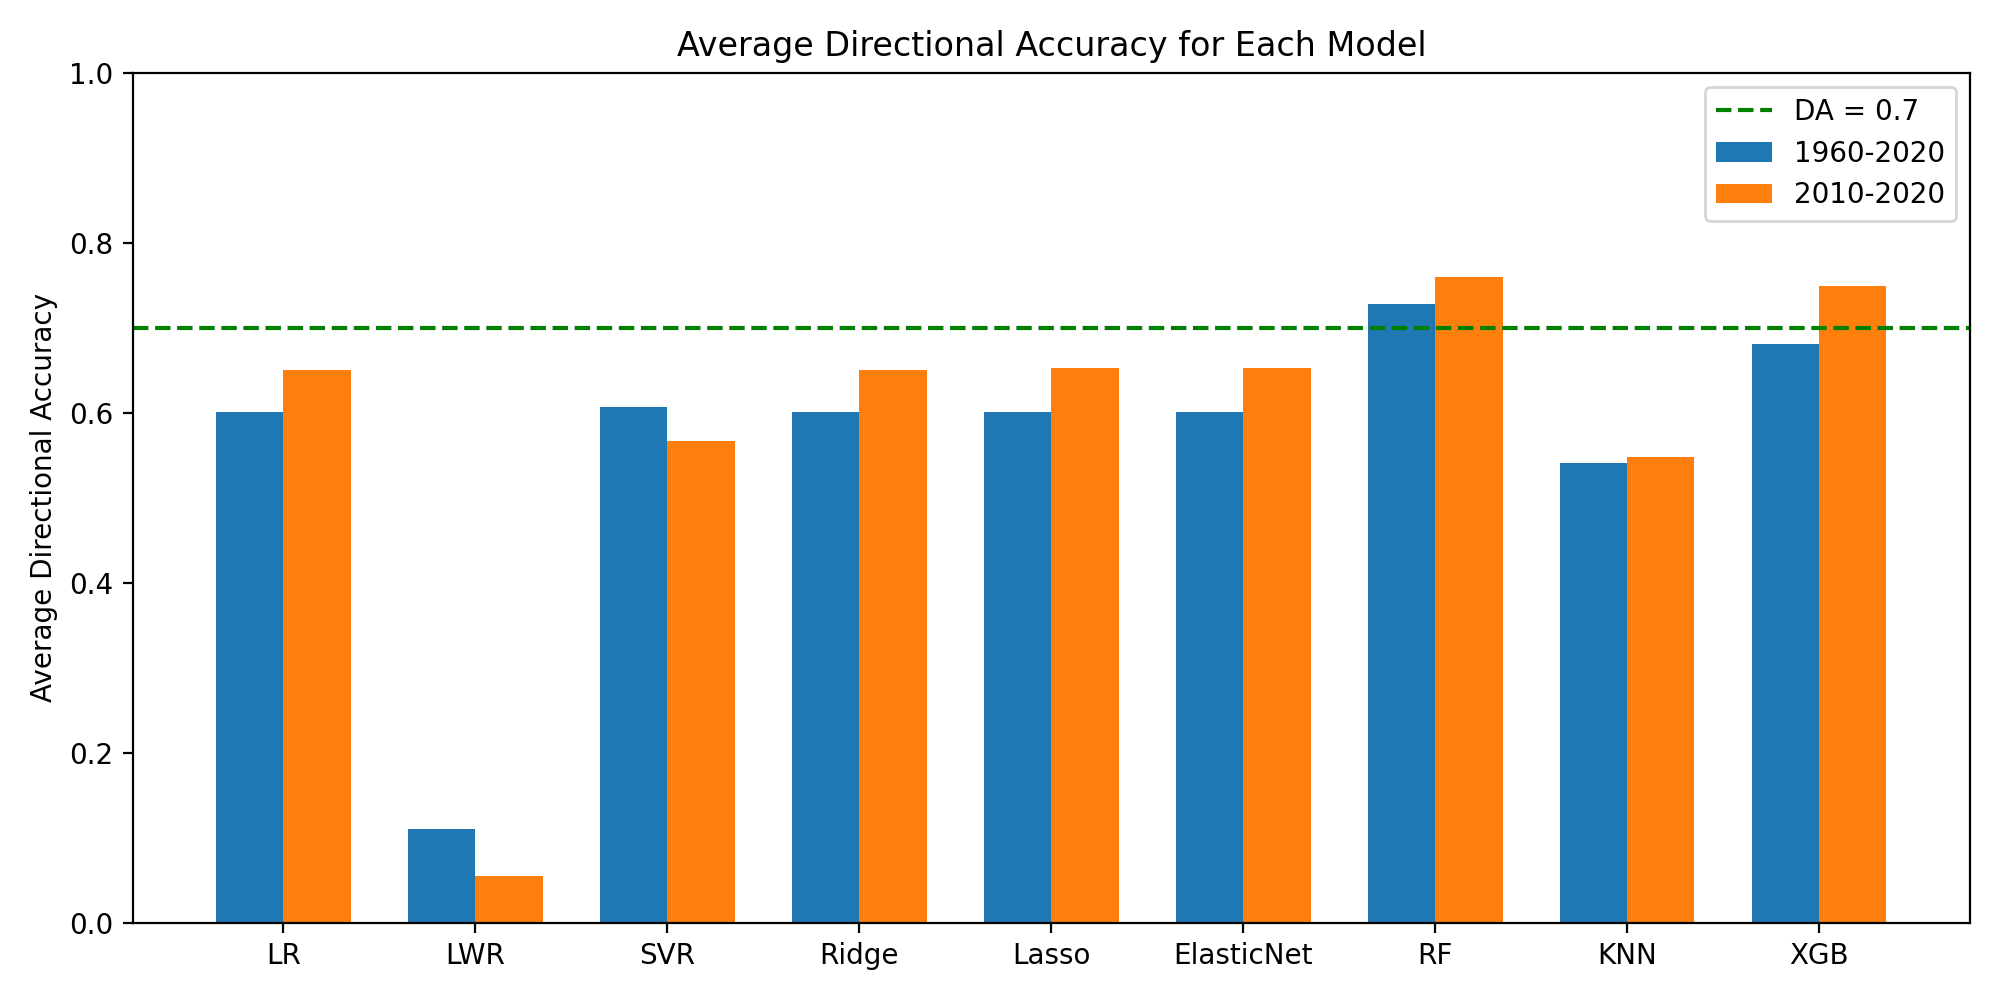
\includegraphics[width=\linewidth]{Average_DA_figure2.png}
        \label{fig:DA}
    \end{subfigure}
    \caption{Comparison of Model Performance: MASE and DA (1960–2020, 2010–2020)}
    \label{fig:model_compare_2}
\end{figure}
\begin{figure}[h]
    \centering
    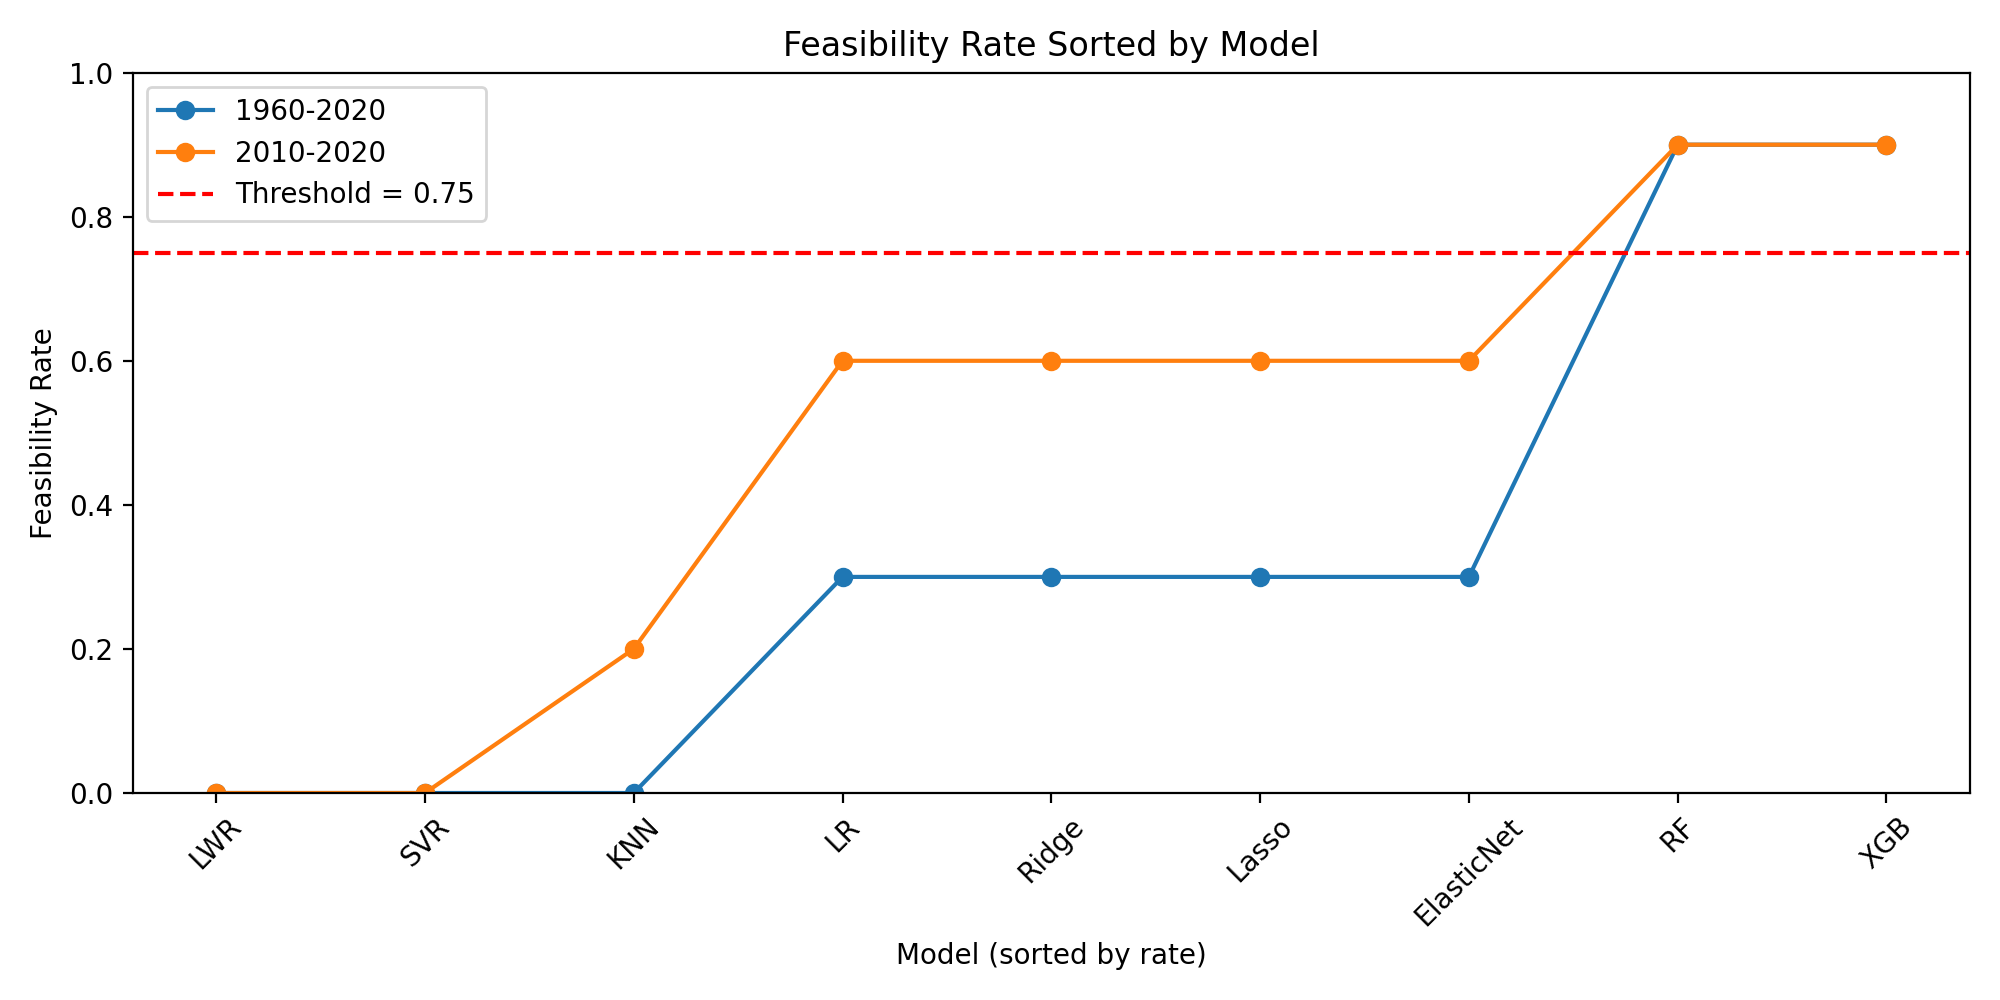
\includegraphics[width=0.8\linewidth]{Feasibility_Rate_Line_Overlay_figure3.png}
    \caption{Feasibility Rate comparison across models in different periods}
    \label{fig:FR}
\end{figure}



We can divide these Machine Learning algorithms into 3 different categories: 
\begin{itemize}
\item RF and XGB have best performances, both of which has a low standardized error, MASE and high $R^2$ and DA, with a feasibility rate of 0.95
\item LR, Ridge, Lasso, ElasticNet have very similar performances, with a feasibility rate of 0.6 (2010-2020) or 0.3 (1960-2020)
\item LWR, SVR, KNN have comparatively low performances. This is in part because the sample size (M = 1220 or 220) is rather small compared to input features (N = 10)
\end{itemize}

\begin{figure}[h]
    \centering
    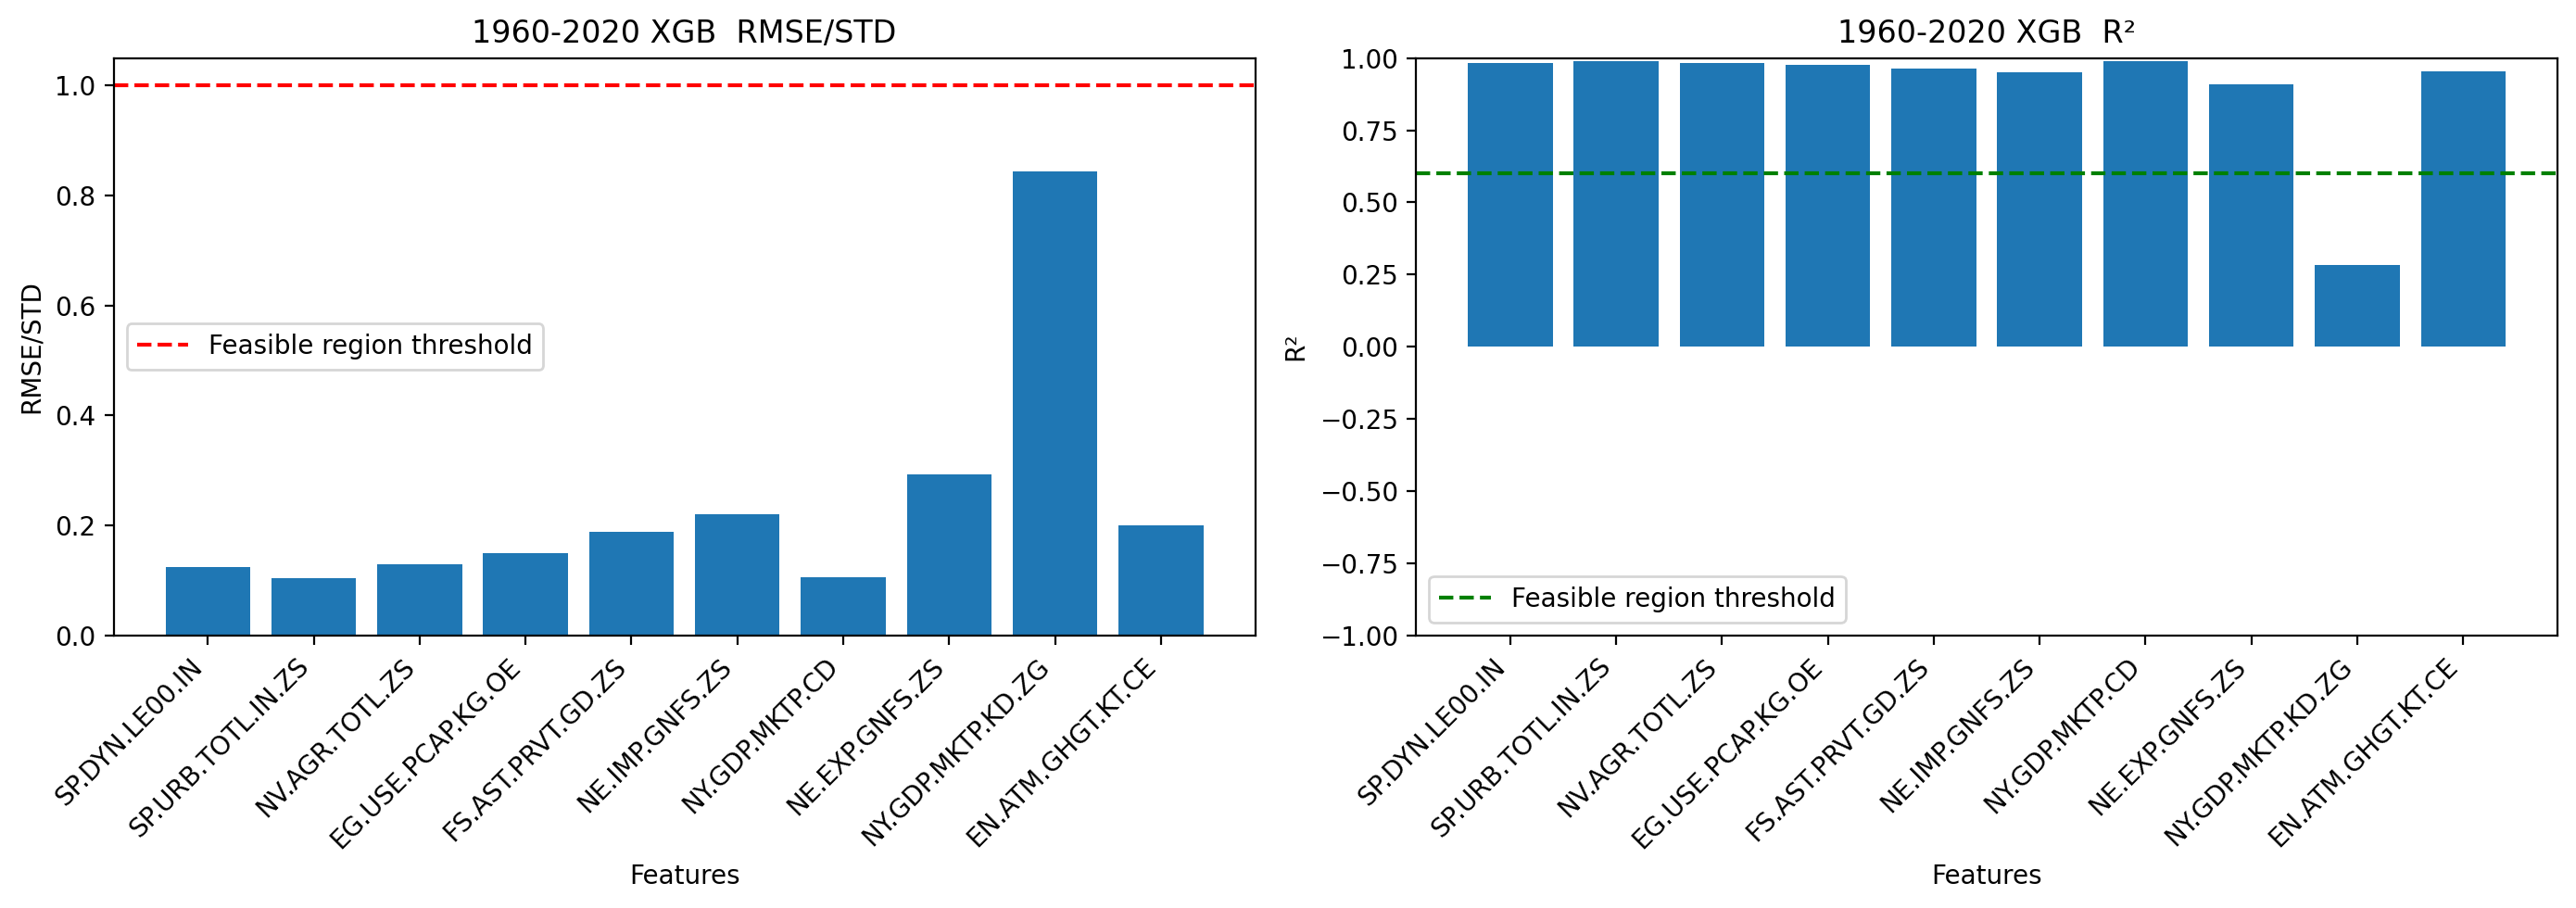
\includegraphics[width=0.95\textwidth]{1960_2020_XGB.png}
    
    \vspace{1em}  % 两图之间的垂直间距

    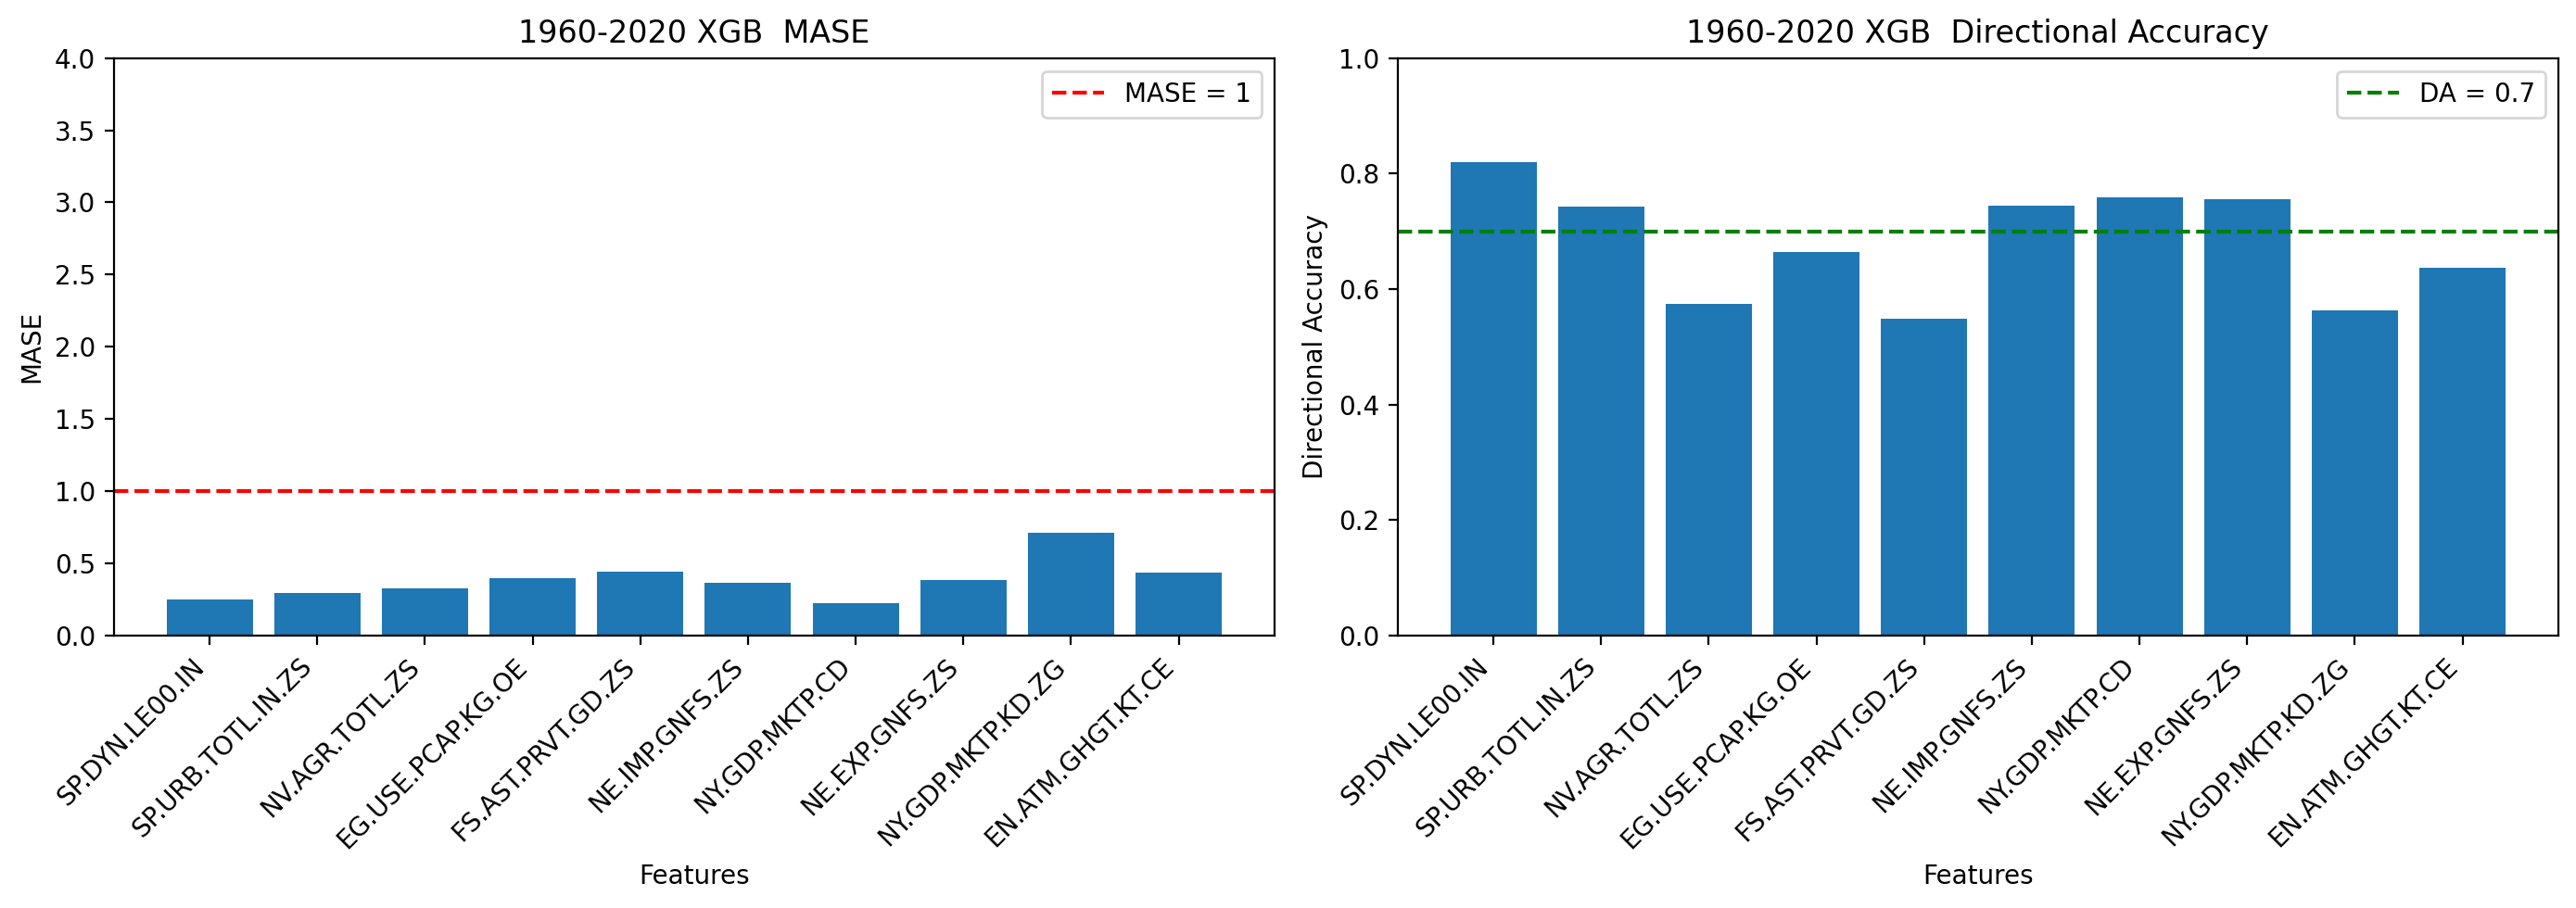
\includegraphics[width=0.95\textwidth]{1960_2020_XGB_mase_da.png}
    
    \caption{Prediction performance of XGBoost for each feature (1960--2020), including RMSE/STD, $R^2$, MASE, and Directional Accuracy.}
    \label{fig:xgb_feature_summary}
\end{figure}
Figure~\ref{fig:xgb_feature_summary} summarizes the prediction performance of XGBoost for each of the 10 selected indicators over the full period (1960--2020). The results indicate that XGBoost achieves high accuracy for most structural indicators, with standardized errors (RMSE/STD) well below 1 and $R^2$ values typically above 0.6. Notably, indicators such as life expectancy, urban population share, and energy use are predicted with particularly high precision. In contrast, GDP growth (annual \%) stands out as the only indicator with consistently poor predictive performance, exhibiting both high error and low explanatory power. The poor predictability of the GDP growth rate compared to other major indicators is primarily due to its intrinsic volatility, exposure to a broad set of unobserved influences, and its weak contemporaneous linkages with slow-moving structural features. This is a well-documented phenomenon in economic modeling ~\cite{Loungani2001, ClementsHendry2002}, where forecasting economic growth remains an exceptionally challenging task.

\subsection{Discussion}
% Discuss the observed performance differences and their economic interpretation.

In this part, we systematically evaluated the cross-predictability of major national indicators using a suite of machine learning algorithms on World Bank panel data spanning six decades. The evaluation leverages four complementary metrics—RMSE/STD, $R^2$, Mean Absolute Scaled Error (MASE), and Directional Accuracy (DA)—along with a composite feasibility rate that captures overall reliability across these dimensions.

Ensemble models such as Random Forest (RF) and XGBoost (XGB) exhibit consistently strong performance across all metrics and both time periods. Their feasibility rates remain the highest among all models, typically exceeding 0.9, reflecting their robustness in capturing complex, nonlinear structures in macroeconomic data.

Support Vector Regression (SVR) and Locally Weighted Regression (LWR), although still the least performant models overall, also show improvements in the recent decade. Their feasibility rates, while remaining low, increase relative to the 1960–2020 baseline, indicating that even the least effective models benefit from more recent data.

Crucially, all ten models exhibit improved performance in the 2010–2020 period. This universal improvement suggests that the recent decade offers more learnable patterns for predictive models. Several factors may explain this. First, the 2010s brought better global data infrastructure, with fewer missing values and more reliable measurements~\cite{jerven2013poor}. Second, structural convergence across economies due to globalization likely increased feature similarity between countries, enhancing cross-national generalizability~\cite{baldwin2016great}. Third, post-crisis macroeconomic policy harmonization and greater institutional stability may have led to more stable, linearizable relationships among indicators~\cite{blanchard2015inflation}.


In contrast, GDP growth (annual \%) consistently shows poor predictive performance due to its volatility, susceptibility to unobserved factors, and weak correlation with slow-moving structural indicators.
This aligns with the Solow model’s view that output growth is partly driven by unpredictable technological shocks, which may not be captured by structural indicators. Moreover, structural transformation theory\cite{Kuznets1971} provides a lens to interpret why some indicators (like agriculture share of GDP) decline in significance over time, reinforcing the importance of context when analyzing indicator relationships.

The feasibility rate offers a valuable heuristic summary of model reliability. By integrating binary thresholds across RMSE/STD, $R^2$, MASE, and DA, it allows for intuitive comparison of how frequently each model yields statistically acceptable forecasts across multiple indicators and periods.

The strong performance of XGBoost and Random Forest can be attributed to their structural advantages in handling economic data. Both models are ensemble tree-based methods capable of capturing complex, nonlinear interactions among predictors—an essential feature given the interdependent nature of macroeconomic indicators. Unlike linear models, these algorithms automatically account for feature interactions without manual specification, enabling them to uncover hidden patterns in high-dimensional datasets. Additionally, they provide built-in measures of feature importance, allowing for greater interpretability and insight into which variables most influence predictions. These characteristics make tree-based ensembles particularly well-suited for datasets with mixed types, multicollinearity, and non-stationarity—common traits in global economic time series.

In summary, the results emphasize not only the superiority of ensemble methods, but also the significant influence of data context: all models—even the weakest—became more effective when trained on recent, high-quality economic data. This highlights the dual importance of methodological choice and temporal data conditions in macroeconomic prediction.

\subsection{Hyperparameter Tuning for XGBoost and Random Forest}

To ensure robust performance from the ensemble models, we conducted hyperparameter tuning for both XGBoost (XGB) and Random Forest (RF) using grid search with 5-fold cross-validation.

For XGBoost, the primary hyperparameters adjusted include:
\begin{itemize}
    \item \texttt{n\_estimators}: Number of boosting rounds.
    \item \texttt{max\_depth}: Maximum depth of each tree.
    \item \texttt{learning\_rate}: Step size shrinkage used in updates.
    \item \texttt{subsample}: Fraction of observations to be randomly sampled for each tree.
    \item \texttt{colsample\_bytree}: Fraction of columns to be randomly sampled for each tree.
\end{itemize}

For Random Forest, the tuning focused on:
\begin{itemize}
    \item \texttt{n\_estimators}: Number of trees in the forest.
    \item \texttt{max\_depth}: Maximum depth of the tree.
    \item \texttt{min\_samples\_split}: Minimum number of samples required to split an internal node.
    \item \texttt{max\_features}: Number of features to consider when looking for the best split.
\end{itemize}

The tuning process selected the best combination of parameters based on cross-validated performance using the feasibility rate as the guiding metric. These optimized settings contributed to the consistent top-tier performance observed in 1960–2020 evaluation.
In addition to tuning global models for each algorithm, we extended the grid search process to each individual indicator. For every target variable, the model was trained and evaluated under multiple parameter combinations, allowing us to select an indicator-specific optimal configuration. 
\begin{figure}[H]
    \centering
    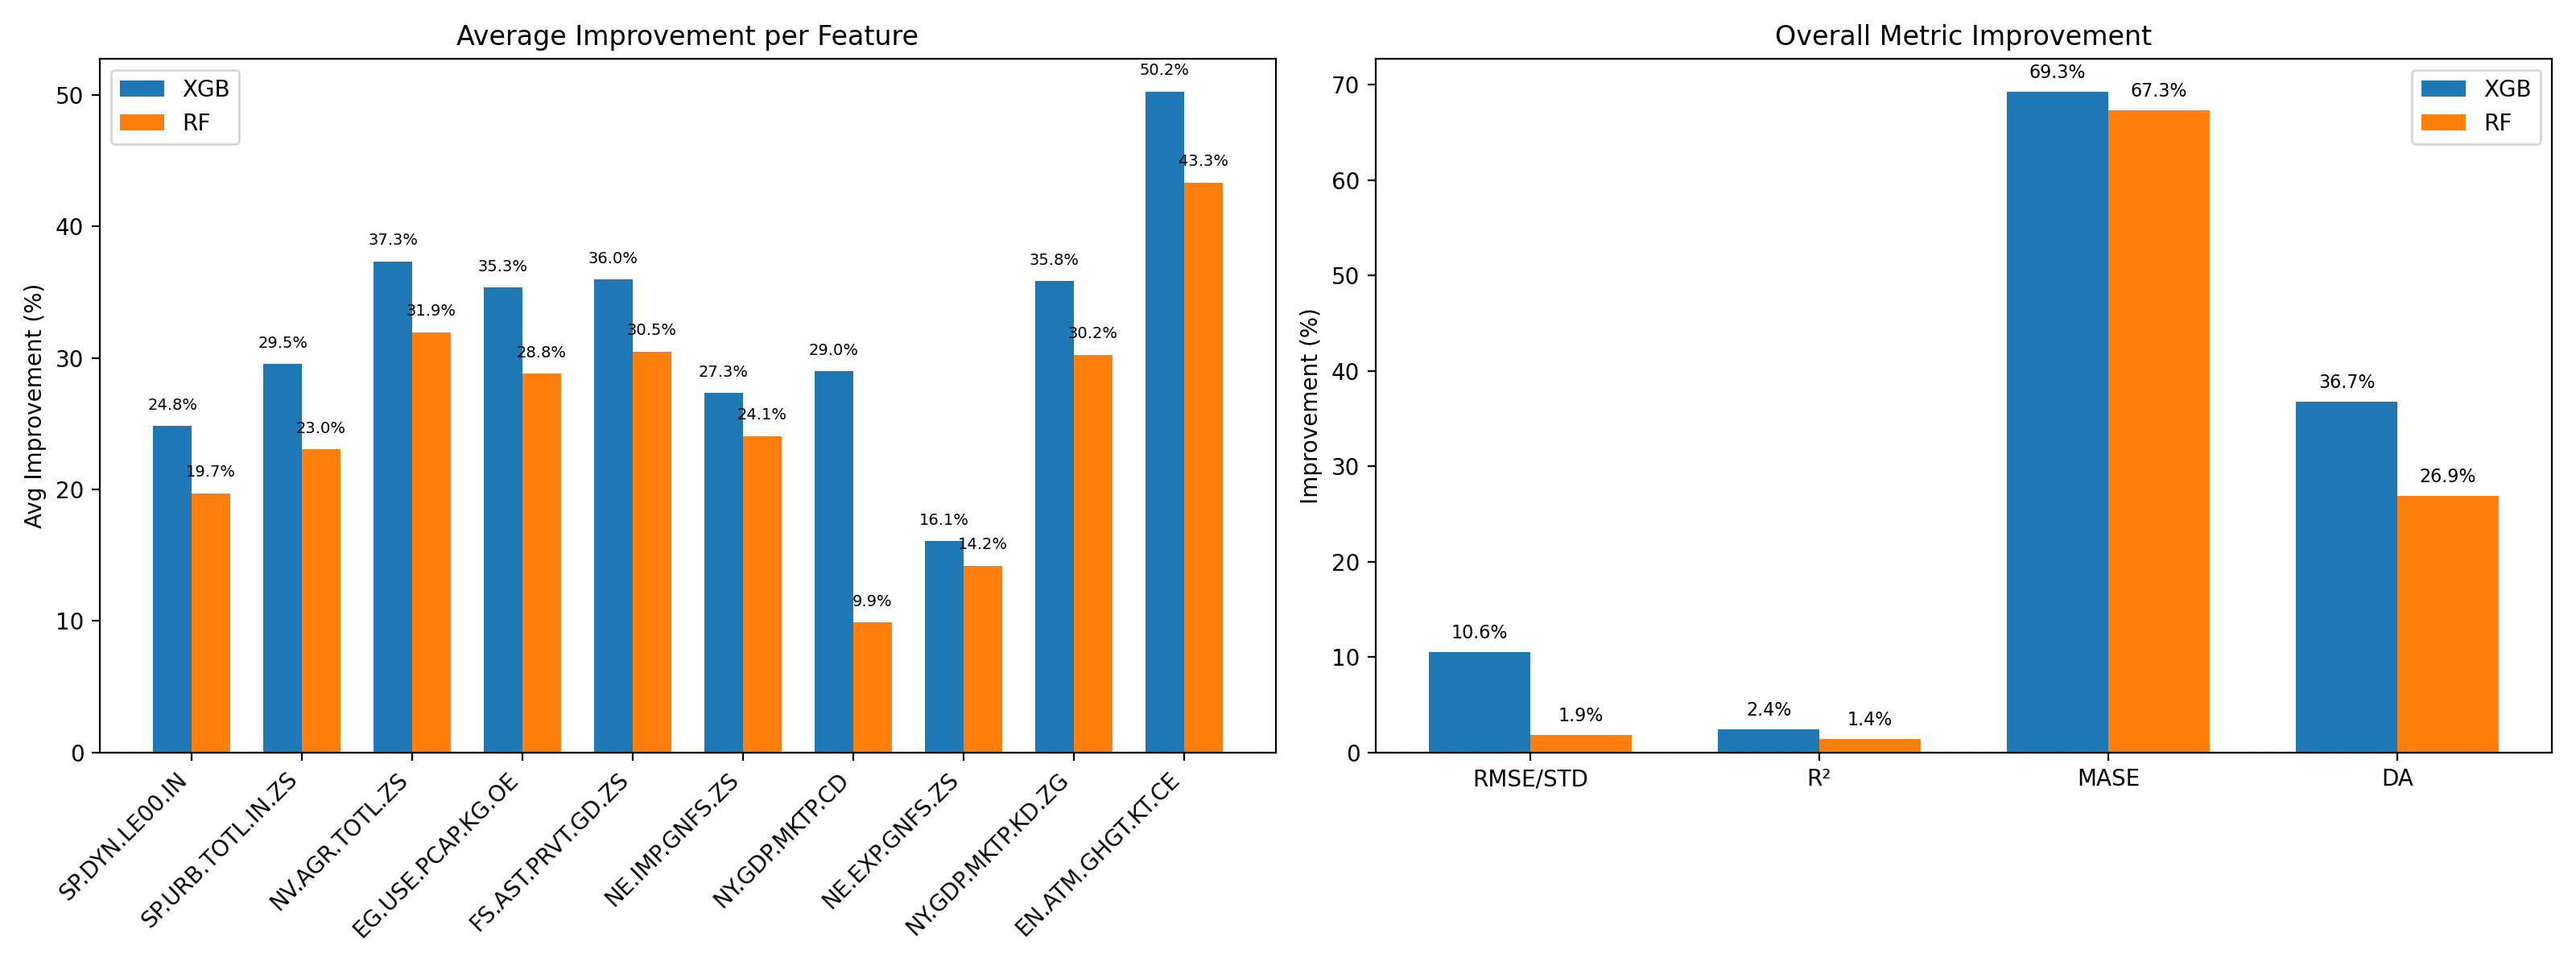
\includegraphics[width=\textwidth]{featurewise_and_modelwise_improvement.png}
    \caption{Feature-wise and overall metric improvement from hyperparameter tuning for XGBoost and Random Forest.}
    \label{fig:tuning_combined}
\end{figure}

Figure~\ref{fig:tuning_combined} provides a detailed visualization of the performance improvements after tuning. The left panel illustrates that while the magnitude of improvement\footnote{Calculated as average of improvement rate of 4 metrics} varies across indicators, all ten features experience a substantial average enhancement, with XGBoost consistently outperforming Random Forest in every case. This confirms that tuning has universal benefit, though its effect size depends on feature characteristics.

The right panel decomposes improvements across the four evaluation metrics. Notably, tuning yields minimal changes in $R^2$ (near 0\%), modest gains in RMSE/STD (ranging from 1\% to 10\%), and substantial improvements in Directional Accuracy (DA), which increase by approximately 30\%--40\%. The most dramatic effect is observed in Mean Absolute Scaled Error (MASE), where XGBoost and Random Forest achieves a nearly 70\% improvement. 
These results highlight how hyperparameter tuning differentially impacts specific model objectives and offer insights into which dimensions of forecast accuracy are most tunable.

\subsection*{Summary of Chapter 4}
In summary, Chapter 4 demonstrates that cross-indicator prediction using machine learning is highly effective for most structural economic indicators, especially when employing ensemble methods such as XGBoost and Random Forest. These models consistently outperform others due to their ability to capture nonlinear interactions and provide robust performance across multiple evaluation metrics. The introduction of the feasibility rate offers a novel and interpretable way to compare model reliability across tasks. Furthermore, hyperparameter tuning significantly enhances accuracy, particularly in directional and scale-sensitive measures. These findings establish a strong foundation for subsequent chapters, which focus on modeling temporal dynamics within countries and generalizing insights across major economies.



\section{Country-Level Time Series Analysis}


\subsection{Temporal Feature Construction}

To enable time series forecasting at the country level, we transformed our panel dataset into a lag-based temporal structure. For each country and each selected indicator, we created lagged features to capture temporal dependencies. Specifically, for a given indicator $F_k$ and time $t$, we generated predictors $F_k(t-1)$, $F_k(t-2)$, and $F_k(t-3)$, effectively encoding three prior observations as input features for predicting $F_k(t)$. 

This approach allows models to infer autoregressive patterns while maintaining a compact feature space. Missing values in lagged sequences were removed through forward-fill interpolation and exclusion of early years where sufficient lags were unavailable. We restricted our modeling to countries with complete post-imputation coverage for at least 30 years, ensuring adequate training depth. This temporal restructuring laid the foundation for consistent forecasting experiments across all indicators and countries.


\subsection{Forecasting Setup}

Our primary forecasting task was to predict the value of each indicator $F_k$ at year $t$ using its lagged values at $t-1$, $t-2$, and $t-3$ for each country individually. This univariate forecasting setup isolates within-indicator dynamics and removes cross-indicator interactions to focus purely on temporal predictability. 

We evaluated three types of models:
\begin{itemize}
    \item \textbf{ARIMA}: A classical statistical model well-suited for univariate time series, used as a benchmark.
    \item \textbf{XGBoost}: A machine learning model capable of learning nonlinear lag structures and complex dynamics.
    \item \textbf{Random Forest (RF)}: An ensemble tree-based method used to capture nonlinear trends and structural breaks.
\end{itemize}

All models were trained in a rolling forecast origin strategy: for each country and indicator, the model was re-trained yearly using all historical data up to year $t$ to forecast $t+1$. This closely simulates real-world forecasting where only past data is available. The models were evaluated using the same four metrics introduced earlier: RMSE/STD, $R^2$, MASE, and Directional Accuracy. For each (country, indicator) pair, we retained both the yearly scores and the overall average to analyze temporal stability and performance consistency.

\subsection{Model Comparison}
% Compare forecasting performance of different time series models on a selected country.
% ------------------------------ Figure 6 Analysis ------------------------------
\subsubsection*{Country-Level Model Feasibility Analysis (Figure 6)}


\begin{figure}[H]
    \centering
    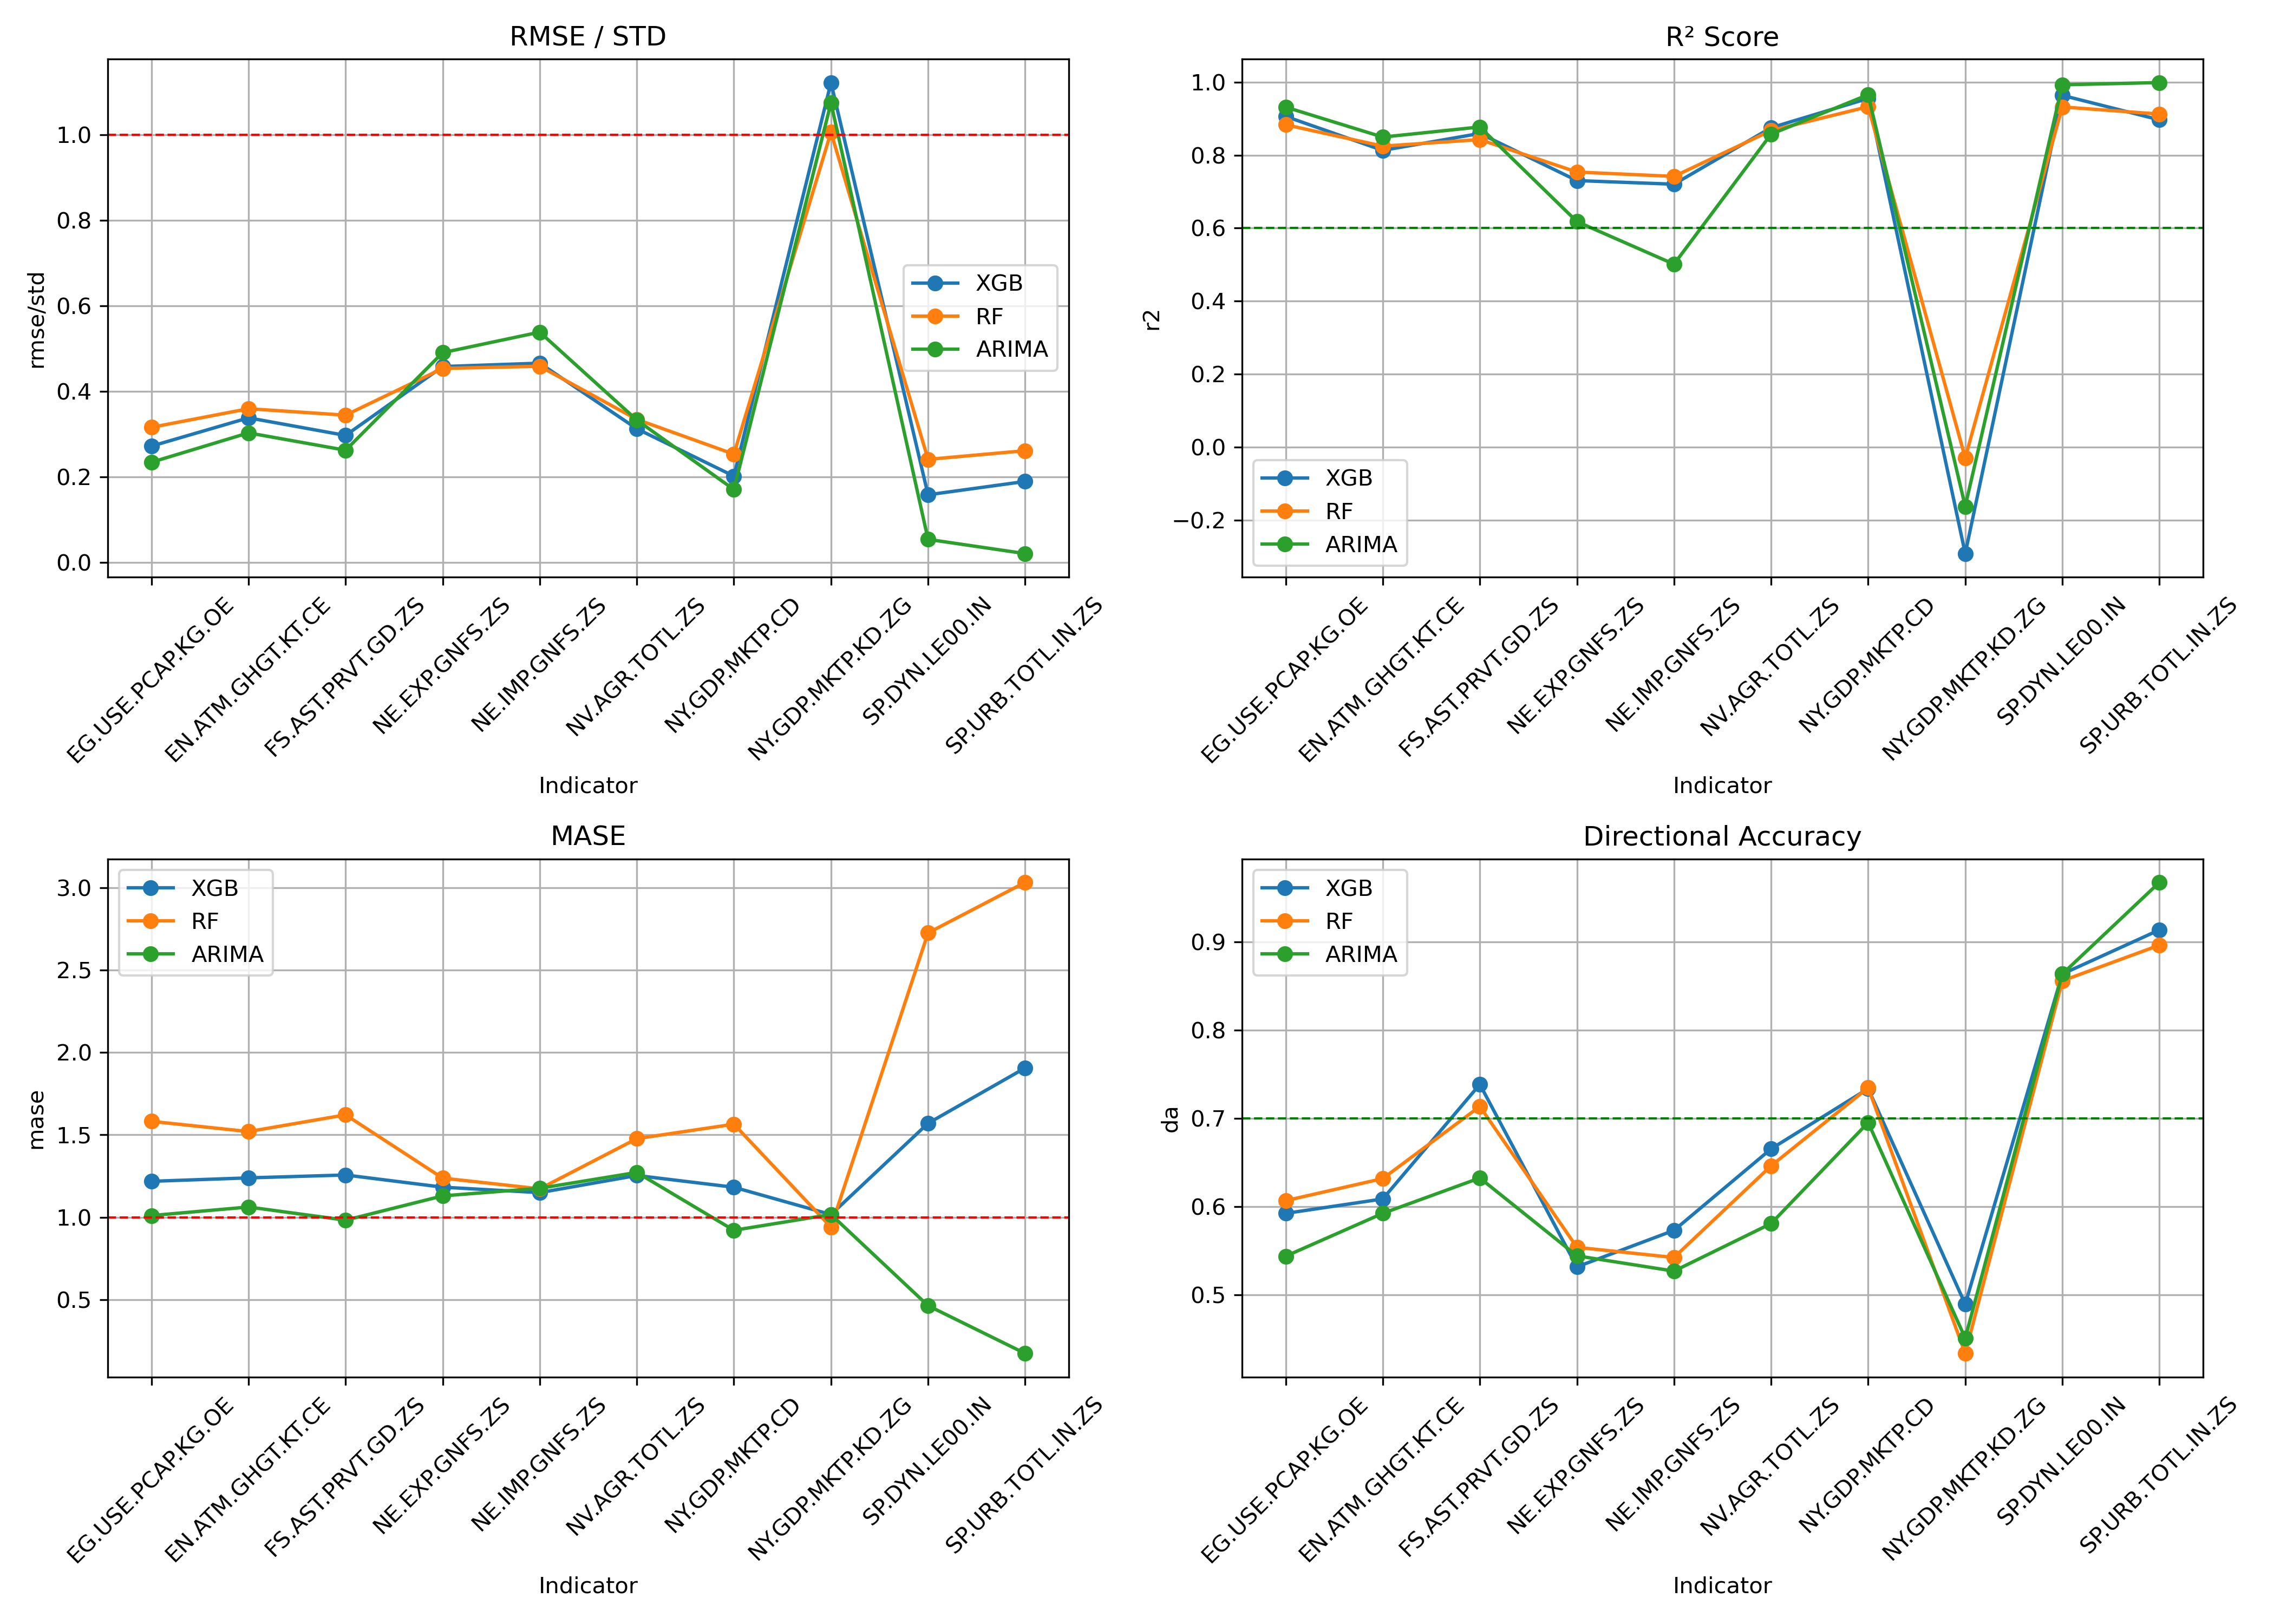
\includegraphics[width=\textwidth]{figure4.png}
    \caption{Comparison of model performance across indicators using four metrics: RMSE/STD, $R^2$, MASE, and Directional Accuracy (DA). }
    \label{fig:indicator_comparison}
\end{figure}

Figure~\ref{fig:indicator_comparison} visualizes the prediction performance of three time series models—XGBoost, Random Forest, and ARIMA—across ten selected macroeconomic indicators. Each subfigure corresponds to one of the four evaluation metrics, with threshold lines indicating feasibility standards.

Across most indicators, all three models achieve standardized errors (RMSE/STD) well below the cutoff of 1. The exception is GDP growth rate, where all models exhibit RMSE/STD above the threshold, confirming its inherent volatility and poor predictability again.

In terms of explanatory power ($R^2$), all three 
models perform strongly on indicators like life expectancy and GDP, often exceeding $R^2 = 0.9$. 
However, for GDP growth, the $R^2$ values drop dramatically, reaching negative values for all three models, reflecting their inability to explain variance in this highly unstable target. This result aligns with long-standing findings in the forecasting literature that GDP growth is notoriously difficult to predict due to its susceptibility to external shocks, technological shifts, and policy discontinuities \cite{Loungani2001, ClementsHendry2002}.

For MASE, ARIMA outperforms both XGBoost and RF on average, particularly for stable indicators like urban population share and life expectancy. However, it should be noted that MASE values for all models tend to exceed the benchmark threshold of 1 on volatile indicators such as GDP growth and trade-related variables. This suggests that while ARIMA benefits from its statistical simplicity, its absolute accuracy remains limited when faced with non-stationary or rapidly shifting macroeconomic environments \cite{Hyndman2006}.

In terms of Directional Accuracy (DA), indicators such as the assets of private sector banks to GDP and overall GDP exhibit strong predictive signals, with all three models achieving DA values above 0.7. Notably, life expectancy and urban population rate emerge as the most directionally stable indicators, with ARIMA approaching near-perfect DA on urbanization—a phenomenon likely driven by the smooth, monotonic trajectories of demographic transitions \cite{Bloom2008, Montgomery2003}. These findings indicate that structural indicators with persistent trends are well suited to directional prediction, even by relatively simple models.

Overall, the heatmap illustrates that while machine learning and statistical models can robustly capture long-term structural patterns, their performance deteriorates on high-volatility targets like GDP growth. This reinforces the need for volatility-aware modeling strategies and careful consideration of economic context when selecting forecast targets.

% ------------------------------ Figure 7 Analysis ------------------------------
\subsubsection*{Indicator-Specific Feasibility by Country (Figure 7)}


\begin{figure}[h]
    \centering
    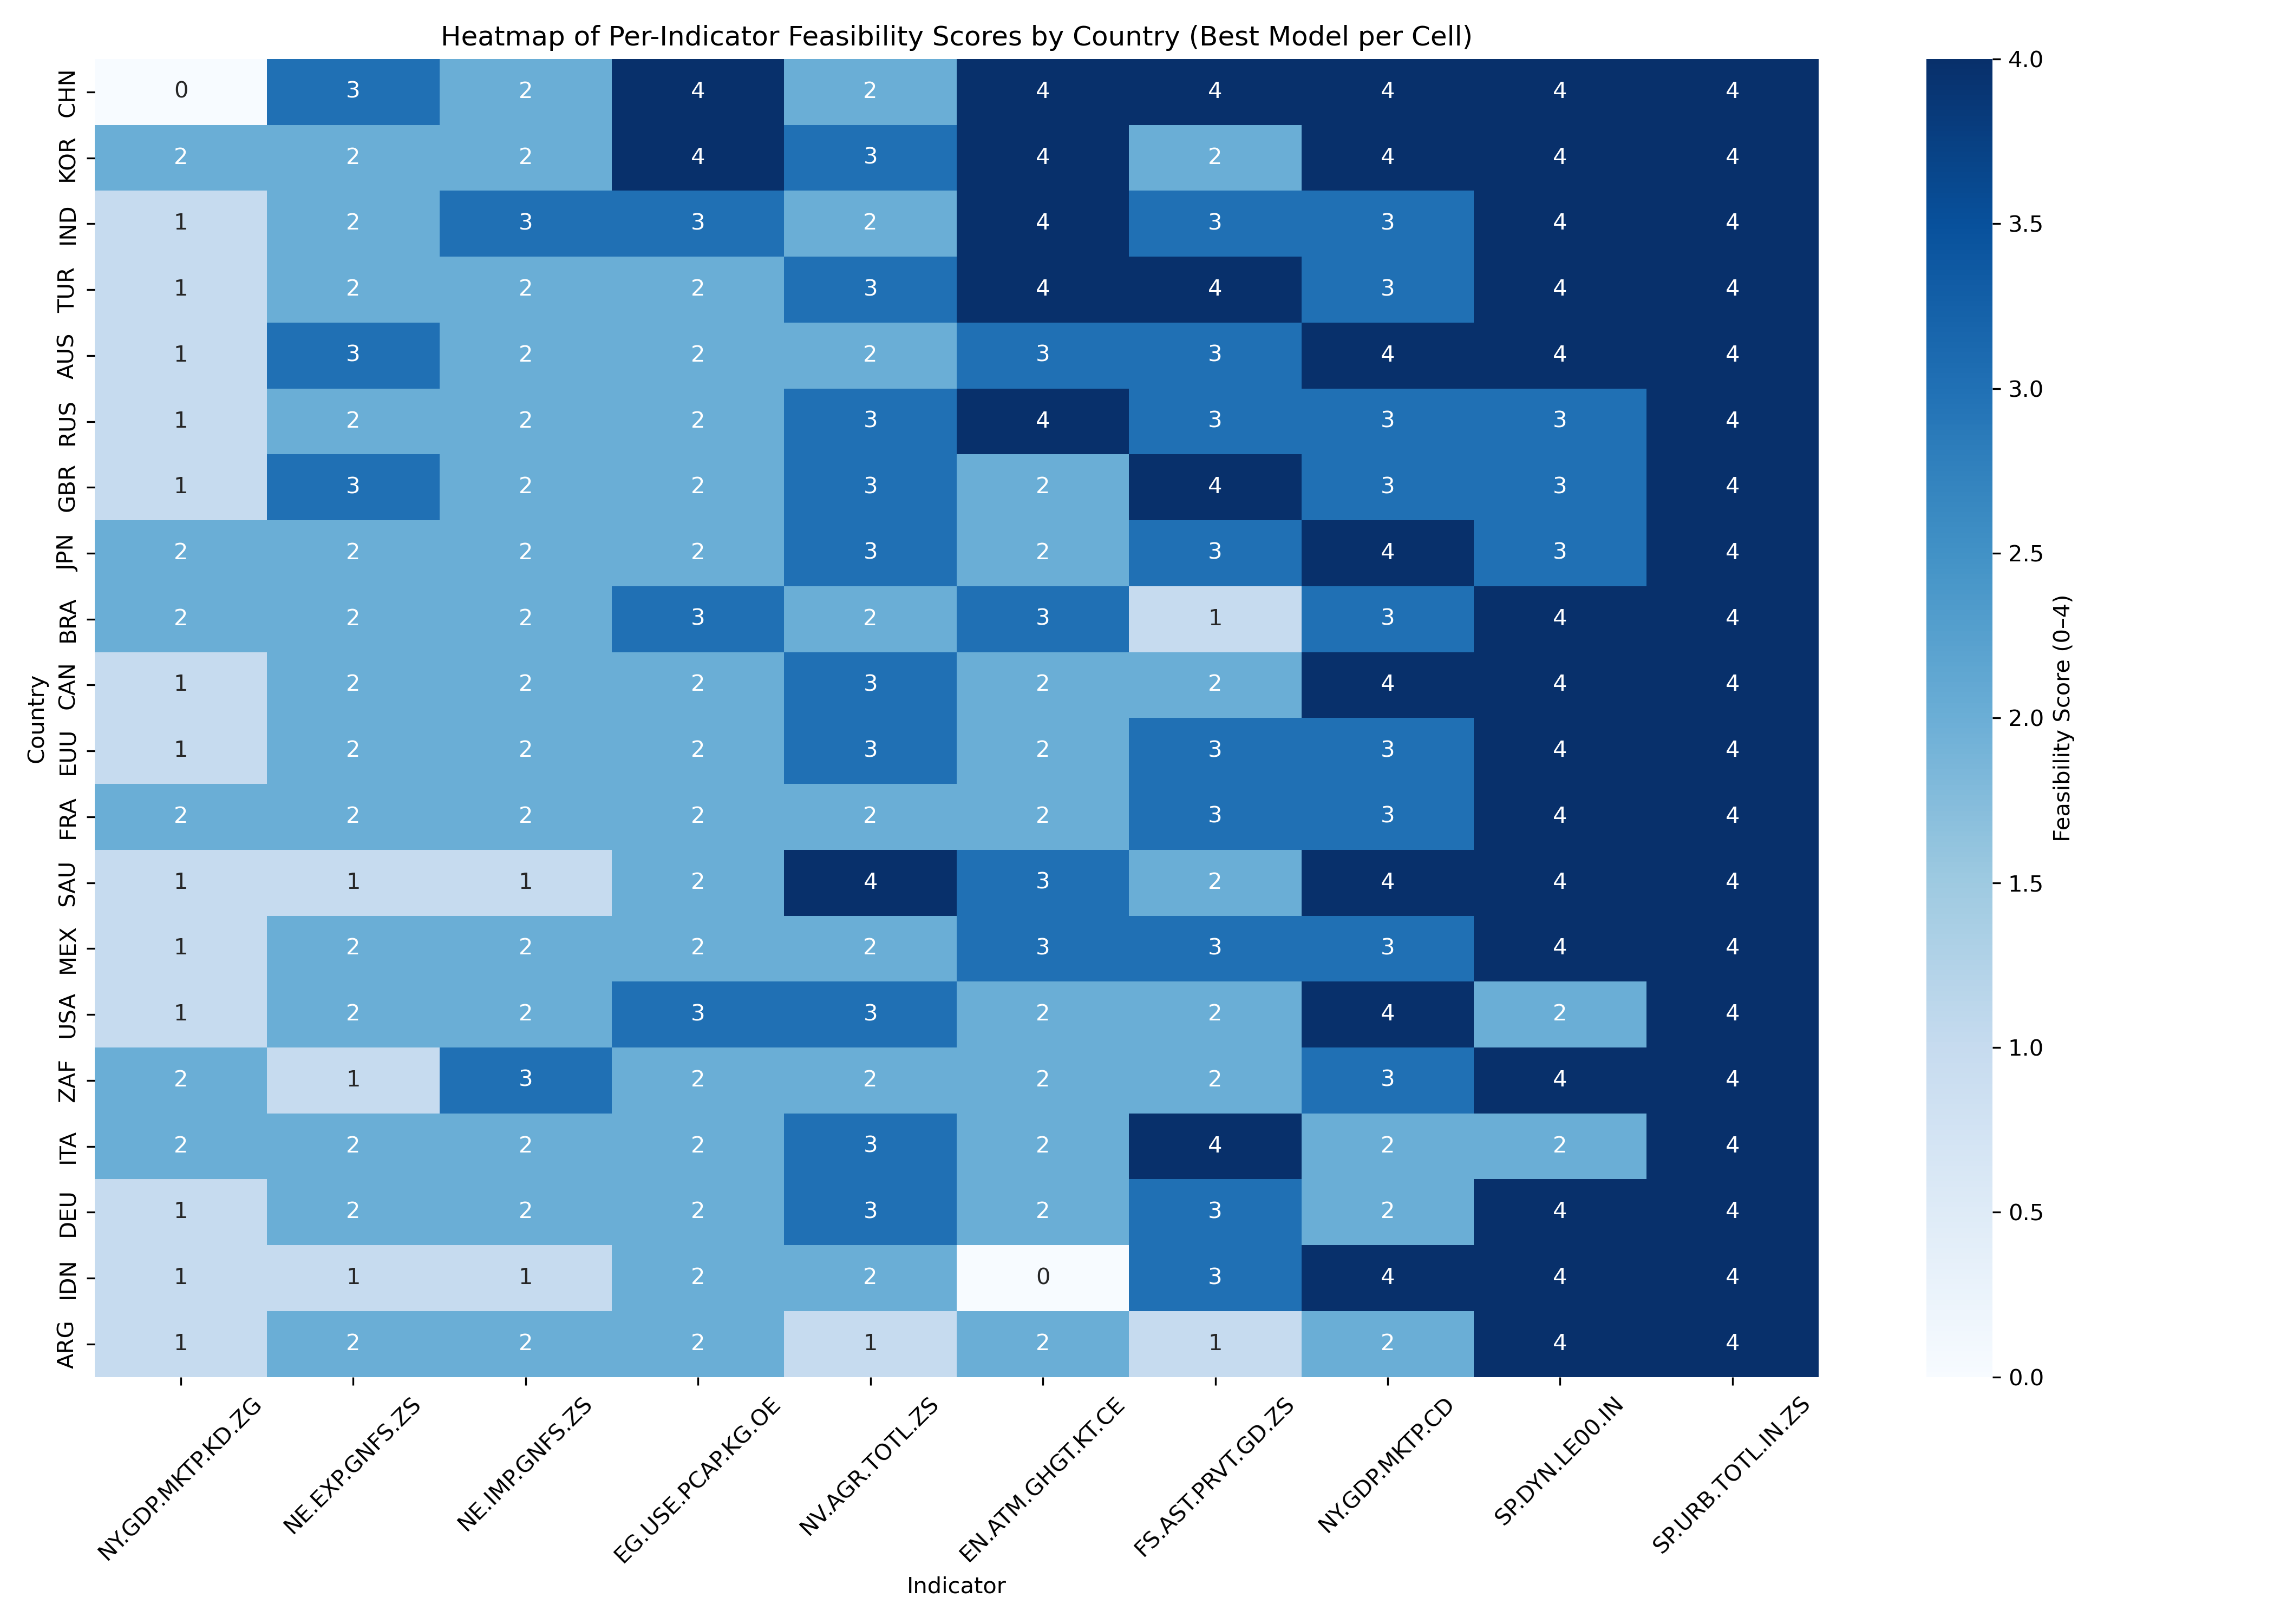
\includegraphics[width=\textwidth]{figure8.png}
    \caption{Heatmap of Per-Indicator Feasibility Scores by Country. For each (country, indicator) pair, we select the best-performing model and report the corresponding feasibility score (0–4). Darker colors indicate more reliable prediction.}
    \label{fig:heatmap_feasibility}
\end{figure}


Figure~\ref{fig:heatmap_feasibility} visualizes the feasibility of predicting macroeconomic indicators across countries using their respective best-performing models. Each cell represents the maximum feasibility score (out of 4)\footnote{For a certain (Country, Model, Indicator), feasbility rate is the sum of $\alpha_i$'s. We have chosen the best model for each (Country, Indicator)} attained by any model for a given (country, indicator) pair. The darker the cell, the higher the reliability of the forecasted value according to our composite metric that combines RMSE/STD, $R^2$, MASE, and Directional Accuracy (DA).

Several key insights emerge:

First, countries such as China, Korea, and India consistently exhibit high feasibility scores across nearly all indicators. Their rows are dominated by the darkest shades, indicating that for these countries, most structural indicators can be predicted with high reliability. This may reflect the availability of cleaner, more complete data, along with stable structural development patterns in these emerging economies \cite{Chen2011development, OECD2019india}.

In contrast, countries such as Argentina, Denmark, and Italy show a wider variance in feasibility across indicators, with many scores clustered around 1–2. This suggests higher volatility or data inconsistency, which impairs model effectiveness even when choosing the best available model.

Second, certain indicators are predictably easier across the board. Urban population\%, life expectancy, and GDP display high scores for almost all countries. These features represent slow-moving structural trends that evolve gradually over time, enabling models to capture their trajectories effectively regardless of the country context.

In contrast, GDP growth\% and trade-related indicators are challenging to predict for most countries, with many feasibility scores below 2. This aligns with findings in forecasting literature that highlight the unpredictability of growth due to sensitivity to shocks, policy regime changes, and latent external factors \cite{Loungani2001, ClementsHendry2002}.

Finally, the heatmap also demonstrates the value of a model-selection strategy. By selecting the best-performing model per cell rather than applying a single model globally, we are able to surface reliable predictions even in challenging data regions. This justifies the use of hybrid or adaptive pipelines in global macroeconomic forecasting tasks.

These results highlight that the feasibility of economic forecasting is a function not only of algorithmic design, but also of indicator volatility, national structural consistency, and the flexibility of the modeling pipeline.

\subsection{Case Study: [Insert Country]}
% Present RMSE, R², plots, and analysis of temporal predictability in that country.

\subsection{Discussion}
% Summarize which indicators are temporally predictable and why. Mention data density or volatility factors.

\subsection{Selection of Major Economies}
% Specify which countries are analyzed (e.g., G7, BRICS).

\subsection{Modeling Setup}
% Define time alignment across countries. Optional: DTW similarity, cross-country lagged features.

\subsection{Cross-National Forecasting}
% Analyze how models trained on one or multiple countries generalize to others.

\subsection{Trend and Volatility Analysis}
% Identify persistent temporal trends vs high-volatility indicators across countries.

\subsection{Discussion}
% Reflect on structural similarity, transferable patterns, and policy relevance of findings.

\section{Conclusion}

This work demonstrates that most major structural indicators of national development are highly predictable from a small set of other key indicators, especially when using ensemble tree-based machine learning models. The exception is GDP growth rate, which remains notoriously difficult to forecast—consistent with macroeconomic theory and previous empirical research.

Our results suggest that, for long-run cross-country comparative analysis, reliable prediction of most economic and demographic indicators is feasible using standard machine learning approaches and open-access datasets. However, caution should be exercised when interpreting models for inherently volatile outcomes such as economic growth. Overall, this study highlights the promise and limitations of data-driven prediction in international development research and points to several avenues for further methodological and substantive refinement.


\section*{Project Repository}
The full code, data preprocessing scripts, and results can be found at: [GitHub link will be inserted here].



\bibliographystyle{unsrt}
\bibliography{references}
\end{document}